% 2006 上海理科卷 Q13；保留原图四顶点的顺序与平行四边形边线。
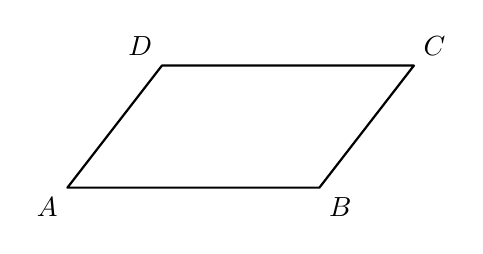
\begin{tikzpicture}[line cap=round,line join=round]
  \coordinate (A) at (0,0);
  \coordinate (B) at (3.2,0);
  \coordinate (C) at (4.4,1.55);
  \coordinate (D) at (1.2,1.55);

  \draw[thick] (A)--(B)--(C)--(D)--cycle;
  \node[below left] at (A) {$A$};
  \node[below right] at (B) {$B$};
  \node[above right] at (C) {$C$};
  \node[above left] at (D) {$D$};
\end{tikzpicture}
